% Exam Template for UMTYMP and Math Department courses
%
% Using Philip Hirschhorn's exam.cls: http://www-math.mit.edu/~psh/#ExamCls
%
% run pdflatex on a finished exam at least three times to do the grading table on front page.
%
%%%%%%%%%%%%%%%%%%%%%%%%%%%%%%%%%%%%%%%%%%%%%%%%%%%%%%%%%%%%%%%%%%%%%%%%%%%%%%%%%%%%%%%%%%%%%%

% These lines can probably stay unchanged, although you can remove the last
% two packages if you're not making pictures with tikz.
\documentclass[11pt]{exam}
\RequirePackage{amssymb, amsfonts, amsmath,amsthm, mathtools, latexsym, verbatim, xspace, setspace}
\RequirePackage{tikz, pgflibraryplotmarks}

% By default LaTeX uses large margins.  This doesn't work well on exams; problems
% end up in the "middle" of the page, reducing the amount of space for students
% to work on them.
\usepackage[margin=1in]{geometry}


% Here's where you edit the Class, Exam, Date, etc.
\newcommand{\class}{Math 1271 - Lecture 050 }
\newcommand{\term}{Spring 2018}
\newcommand{\examnum}{Quiz VII}
\newcommand{\examdate}{3/22/18}
\newcommand{\timelimit}{20 Minutes}
\DeclarePairedDelimiter\abs{\lvert}{\rvert}%
% For an exam, single spacing is most appropriate
\singlespacing
% \onehalfspacing
% \doublespacing

% For an exam, we generally want to turn off paragraph indentation
\parindent 0ex
\def\changemargin#1#2{\list{}{\rightmargin#2\leftmargin#1}\item[]}
\let\endchangemargin=\endlist 
%%\usepackage{pgfplots}
%%\pgfplotsset{my style/.append style={axis x line=middle, axis y line=
%		middle, xlabel={$x$}, ylabel={$y$}, axis equal,width=\textwidth }}
%	\pgfplotsset{every x tick label/.append style={font=\small, yshift=0.5ex}}
%	\pgfplotsset{every y tick label/.append style={font=\small, xshift=0.5ex}}
	\renewcommand{\d}[1]{\ensuremath{\operatorname{d}\!{#1}}}
	\newcommand{\pydx}[2]{\frac{\partial #1}{\newcommand\partial #2}}
	\newcommand{\dydx}[2]{\frac{\d #1}{\d #2}}
	\newcommand{\ddx}[1]{\frac{\d{}}{\d{#1}}}
	\newcommand{\evat}[3]{\left. #1\right|_{#2}^{#3}}
	\newcommand{\restr}[2]{\evat{#1}{#2}{}}
\begin{document} 

% These commands set up the running header on the top of the exam pages
\pagestyle{head}
\firstpageheader{}{}{}
\runningheader{\class}{\examnum\ - Page \thepage\ of \numpages}{\examdate}
\runningheadrule

\begin{flushright}
\begin{tabular}{p{2.8in} r l}
\textbf{\class} & \textbf{Name (Print):} & \makebox[2in]{\hrulefill}\\
\textbf{\term} &&\\
\textbf{\examnum} &&\\
\textbf{\examdate} &&\\
\textbf{Time Limit: \timelimit} & Section & \makebox[2in]{\hrulefill}
\end{tabular}\\
\end{flushright}
\rule[1ex]{\textwidth}{.1pt}

You may \textit{not} use your books, notes, graphing calculator, phones or any other internet devices on this exam. Please show all work clearly and legibly.\\

%You are \textbf{required} to justify your answers rigorously on each problem on this quiz. Supporting evidence and/or informal justification may be redeemed for partial credit.\\
\hspace*{12cm}\begin{minipage}[t]{2.3in}
\vspace{0pt}
%\cellwidth{3em}
\gradetablestretch{2}
\vqword{Problem}
\addpoints % required here by exam.cls, even though questions haven't started yet.	
\gradetable[v]%[pages]  % Use [pages] to have grading table by page instead of question

\end{minipage}
%\newpage % End of cover page

%%%%%%%%%%%%%%%%%%%%%%%%%%%%%%%%%%%%%%%%%%%%%%%%%%%%%%%%%%%%%%%%%%%%%%%%%%%%%%%%%%%%%
%
% See http://www-math.mit.edu/~psh/#ExamCls for full documentation, but the questions
% below give an idea of how to write questions [with parts] and have the points
% tracked automatically on the cover page.
%
%
%%%%%%%%%%%%%%%%%%%%%%%%%%%%%%%%%%%%%%%%%%%%%%%%%%%%%%%%%%%%%%%%%%%%%%%%%%%%%%%%%%%%%


\begin{questions}

% Basic question
%\vspace*{-130pt}
\addpoints
% Find the real numbers within the interval $I$ at which $f$ is \emph{not} continuous. State whether $f$ is continuous from the right, the left, or neither.
%\begin{parts}
%\part[1] $\displaystyle{f(x)=\frac{1}{x^2+4x-21}}$\hfill $I=(-\infty,\infty)$\vskip1.5mm
%\part[1] $\displaystyle{f(x)=\frac{\sin{\frac{x}{2}}}{\cos{2x}}}$\hfill $I=[-\pi,\pi]$\vskip1.5mm
%\part[1] $\displaystyle{f(x)=\begin{cases}2^x&x\leq 3\\-3x+17&3<x\leq 4\\\frac{1}{\sqrt{x-3}}&x>4
%	\end{cases}}$\hfill $I=(-3,8)$
%\end{parts}
\vspace*{-120pt}
\question[8]\begin{changemargin}{0pt}{137.4803pt}
 A shoebox (with no lid) is to have a rectangular base with length double its width and an open top. You have 450 in${}^2$ of cardboard from which to make the box. What dimensions maximize its volume?\end{changemargin}\vspace{60pt}
\begin{proof}[Response]
	We draw the picture of figure one (note that the box is three-dimensional):\begin{figure}[h!]\begin{centering}
		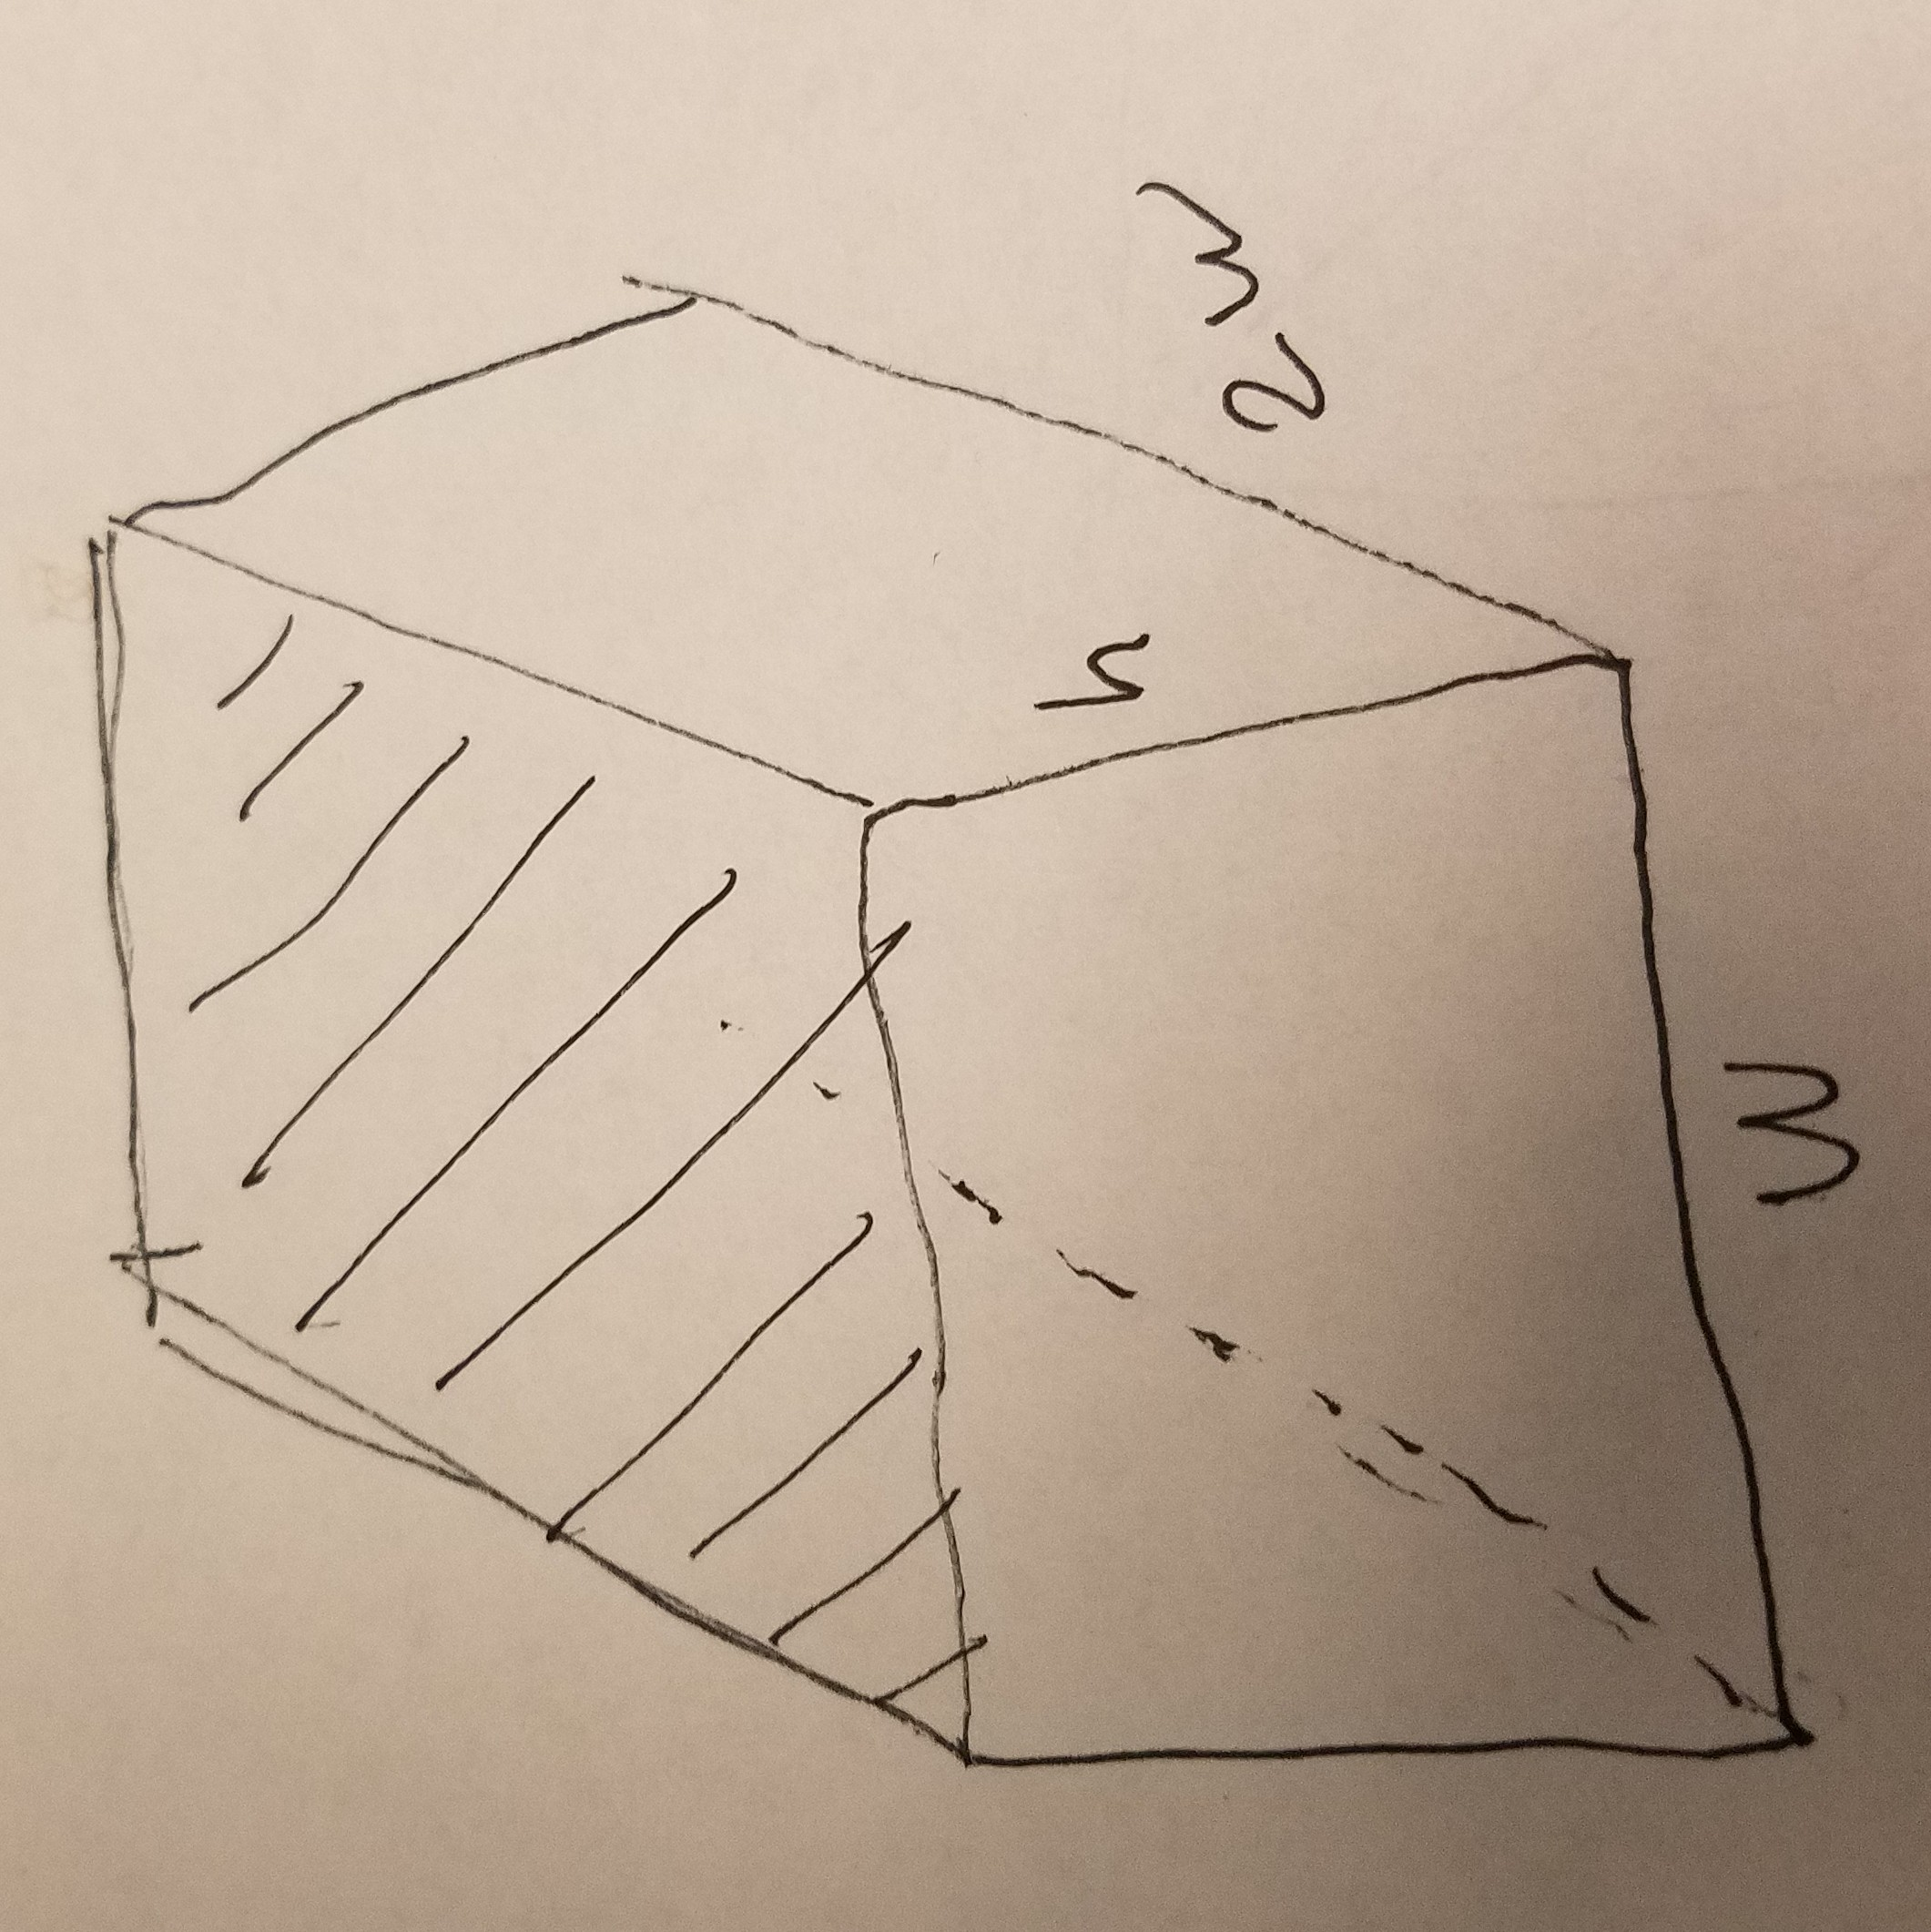
\includegraphics[scale=.1,angle=270]{shittybox}\caption{A box with base-length twice its width and an open top}\end{centering}
	\end{figure}

The quantity we must maximize is $V=2w^2h$. Our given constraint is that the surface area is 450 in${}^2$. Going side-by-side, we calculate that the surface area is $2w^2+2wh+2*2wh=2w^2+6wh$, so we have the relation $450=2w^2+6wh$. We also have the endpoints $h\geq 0$, $w\geq 0$. We use our relation to find $$h=\frac{450-2w^2}{6w}=75w^{-1}-\frac{1}{3}w$$
Then, we use this to adjust our endpoint:
\begin{align*}
	h&\geq 0\\
	\implies 75w^{-1}-\frac{1}{3}w&\geq 0\\
	\implies 75-\frac{1}{3}w^2&\geq 0\\
	\implies 75&\geq \frac{1}{3}w^2\\
	\implies 225&\geq w^2\\
	\implies 15&\geq w
\end{align*}
Thus, we are optimizing on the interval $w\in [0,15]$. Finally, we use our form for $h$ to put $V$ in terms of $w$:
$$V(w)=2w^2h=2w^2(75w^{-1}-\frac{1}{3}w)=150w-\frac{2}{3}w^3$$
To find critical points, we find $V'(w)=150-2w^2$. We set it equal to $0$:
\begin{align*}
	0&=150-2w^2\\
	\implies 2w^2&=150\\
	\implies w^2&=75\\
	\implies w=\sqrt{75}=5\sqrt{3}
\end{align*}
We note as well that $V(0)=V(15)=0$. Since $w=5\sqrt{3}$ is our only critical point and $V(5\sqrt3)>0$, we have that it is our maximizing width. We then calculate for our maximizing $h$:\begin{align*}
	h&=\frac{75}{w}-\frac{w}{3}\\
	&=5\sqrt{3}-\frac{5}{3}\sqrt{3}=\frac{10\sqrt{3}}{3}
\end{align*}
\end{proof}
\newpage
\addpoints
\question Let $f(x)=x^3+x^2-2x-2$\begin{parts}\part[6] Determine the intervals of concavity and inflection points for $f$. \begin{proof}[Response] We find that $f''(x)=6x+2=6(x+\frac{1}{3})$. Thus, $f$ is concave down on $(-\infty,-\frac{1}{3})$ and concave up on $(-\frac{1}{3},\infty)$ with an inflection point at $x=-\frac{1}{3}$. 
		\end{proof}\vspace{1cm}
\part[6] Use Newton's method to estimate a \textbf{critical point} of $f$ to five decimal places with starting point $x_1=1/2$. \\\emph{(Hint: stop and read this question again before you start working on your answer).}
\begin{proof}[Response]
	Note that finding a \textbf{critical point} equates to finding a \textbf{zero} of the \textbf{derivative.} Thus, our set-up should be $$x_i=x_{i-1}-\frac{f'(x_i)}{f''(x_i)}$$
	Using this, we find:
	\begin{align*}
		x_1&=.5\\
		x_2&=.55\\
		x_3&=.548585\\
		x_4&=.548584\\
	\end{align*}
Thus, the answer we are looking for is $x\approx .54858$.
\end{proof}
 \end{parts}
%\vskip70mm
%\addpoints
%\question
%%\noaddpoints
%Evaluate the following limits. Justify your response carefully and fully. 
%\part[2] $\displaystyle{\lim_{x\to \infty} \frac{\sin^2(x)}{2x^2+1}}$
%\vspace{1.3in}
%\part[2] $\displaystyle{\lim_{x\to -\infty} \frac{3x^3+2x-1}{\abs{x^3+2x^2+1}}}$ 
%\end{parts}
%%\addpoints
\addpoints

\end{questions}
\end{document}